% Introduction
\section{Introduction}

%%%%%%

% Cite:
% Wireless sensor networks	#yick2008wireless
% Mobile campus networks 	#hernandez2005comparative
% Mobile gaming community	#cunningham2002optimizing
% Energy-efficient network	#jones2001survey
% Internet of things 			#qin2014software

% The cite of the existing algorithms are listed in related work

%%%%%%

% Paper Logic Flow
% P1-P2 Background
% P3-P6 motivation
% P7-P11 contribution
% P12 structure

% P1:    
% General background
% The situation&scenario our research applies to
The growing interest in the Internet of Things (IoT) has resulted 
in a number of wide-area deployments of wireless networks \cite{qin2014software},
such as wireless sensor networks \cite{yick2008wireless}, mobile campus networks 
\cite{hernandez2005comparative}, mobile gaming community \cite{cunningham2002optimizing}, etc.
All these networks possess multi-hop and large-scale characteristics obviously.

% P2: 
% Why NB problem is related and important to the background in P1  
% Define what is neighbor and what is neighbor discovery problem
% A brief introduction of the existing works and explain deterministic and probabilistic with one sentence each
Neighbor discovery is a fundamental step of constructing a wireless network, based on 
which the network can implement further applications such as routing and broadcasting.
The core target is for each node in the network to discover the nodes in its radio sensing range 
with one-hop communication, which are called neighbors. 
A number of existing methods \cite{dutta2008practical,kandhalu2010u,
bakht2012searchlight,sun2014hello,chen2015heterogeneous,
wang2015blinddate,qiu2016talk,mcglynn2001birthday,
vasudevan2009neighbor,you2011aloha,song2014probabilistic} have been proposed 
to deal with this issue, some of which are based on deterministic techniques, 
those turn on the radio with deterministic sequences,
 while others are probabilistic approaches, those turn on the radio with different probabilities.


% P3:
% Crucial problem:  collision issue in a partially-connected network
% What is a practical network model and define what is a partially-connected network
Unfortunately, despite great efforts, neighbor discovery remains an open problem.
The crucial issue lies in the collision situation in the large-scale networks.
In a large-scale network, each node is only able to sense the 
nodes located nearby itself based on received signal strength \cite{wang2013gaussian}.  
We call this network connection structure as partially-connected networks.


% P4: 
% What issues will occur, if transferring the deterministic methods to the partially-connected network
As for the deterministic approaches, they only deal with the neighbor discovery problem for two nodes.
When transferred to partially-connected networks,
they can not solve the collision issue when more than one neighbors are transmitting simultaneously. 

% P5:
% What issues will occur, if transferring the probabilistic methods to the partially-connected network
Relatively, probabilistic approaches are designed for the networks where all the nodes can communicate with each other.
They can well deal with multiple nodes discovery but only consider
the network is fully-connected, the topology of which is a complete graph. 
Therefore the probability adopted in these approaches can not be desirable 
and thus can not reduce the collision efficiently.


% P6: 
% Summarize and highlight the crucial issue : partially-connected network and practical distribution
% Give the reason why it is import to take the distribution into consideration
To our best knowledge, no relevant researches have focused on neighbor discovery problem
in the partially-connected networks. More practically, in a wireless network the distribution of 
nodes' deployment consequently plays a vital role in determining the intrusion detection capability of a sensor node.
Thus the distribution of the nodes in the network needs to be fully taken into 
consideration.

% P7:
% Our solution/contribution : we propose Alano algorithm based on the distribution of nodes for the partially-connected networks
In this paper, we propose Alano\footnote{Alano is the god of luck in Greek mythology.}, 
a nearly optimal probability based algorithm to discover neighbors in partially-connected networks. 
As fully studied in \cite{wang2013gaussian} , the nodes in wireless sensor networks are likely to 
follow a uniform or a Gaussian distribution as showed in Fig. \ref{distribution}, 
depending on the specific network applications, which is taken in consideration of the proposed Alano algorithm.

 
 \begin{figure}[!t]
\centering
\subfigure[uniform distribution]{\includegraphics[width=1.7in]{./Figure/uniform.eps}}
\vspace{0.03in}
\subfigure[Gaussian distribution]{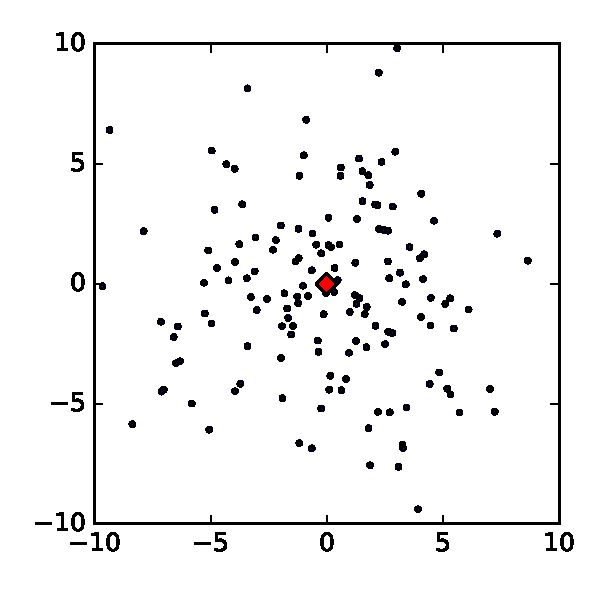
\includegraphics[width=1.7in]{./Figure/normal.eps}}
\caption{WSN deployments following uniform and Gaussian distribution.}
\label{distribution}
%\vspace{-0.2in}
\end{figure}


% P8: 
% A special type of partially-connected networks: energy-efficient network
In addition, among the partially-connected networks, there is a special 
type named energy-efficient network \cite{jones2001survey}.
Wireless sensor network is a typical energy-efficient network that all the sensor nodes have to maintain 
strict power budgets to attain years of lifetime\cite{dunkels2011contikimac}.
Duty cycle mechanism, the fraction of time the radio is turned on, is 
utilized to raise the power-awareness of the nodes in the network.
Correspondingly, the neighbor discovery process 
needs adjustments to deal with the dilemma between 
a balance of energy-efficiency and low-latency.


% P9: 
% For energy-efficient networks, we propose RDS-Alano in global duty cycle scenario 
% and TP-Alano in the local duty cycle scenario.
For energy-efficient networks, we design deterministic methods
to align the wake-up time slot between the neighbors to achieve lower latency bound.
Specifically, We propose RDS-Alano algorithm for the global duty cycle scenario, where 
all the nodes share a identical duty cycle $\theta$ and TP-Alano for the
local duty cycle scenario where each node holds a distrinct duty cycle $\theta_i$. 


% P10:
% Simulation results support our high performance
Our simulation under the practical distribution of networks 
\cite{wang2013gaussian} shows the proposed Alano algorithm
holds significant strengths than the state-of-the-art methods,
based on the evaluation of speed, quality and scalability.
Alano achieves 31.35\% to 32.32 times lower latency
and has higher discovery rate during the whole course of neighbor discovery, 
with either global or local duty cycle in both uniform and Gaussian distribution.
When the number of nodes increases and the network becomes denser, 
Alano still keeps its high performance. 


% P11:
% Contribution summarize
The main contributions of this paper are summarized as follows:
\begin{itemize}
\item[1)] We model the distribution of node deployment with mathematical analysis 
and analyse the expectation number of neighbors of a node in uniform distribution and Gaussian
distribution.
\item[2)] We propose Alano, a low-latency strategy to achieve neighbor discovery process
in a partially-connected network.
\item[3)] We propose a Relaxed DifferenceSet based Alano algorithm (RDS-Alano) 
to achieve low-latency neighbor discovery process in the global duty cycle scenario. 
\item[4)] We propose a Traversing Pointer based Alano algorithm (TP-Alano) 
achieve low-latency neighbor discovery process in the local duty cycle scenario. 
\end{itemize}


% P12:
% Remaining structure
The remainder of the paper is organized as follows.
The next section highlights some related work and 
puts forward some serious problems. 
Some notion definitions and the system model are given in Section
\ref{sectionmodel}. 
We analyse the node's expectation number of neighbors and 
propose Alano algorithm in \ref{PCN} as a foundation.
Section \ref{EEN} describes the RDS-Alano algorithm for global
duty cycle scenario and TP-Alano algorithm for local duty cycle scenario
respectively in energy-efficient networks.
We have conducted extensive simulations, and the results are shown in Section
\ref{Evaluation}. Finally, we conclude the paper in Section
\ref{Conclusion}.

